\begin{figure*}[t]
\centering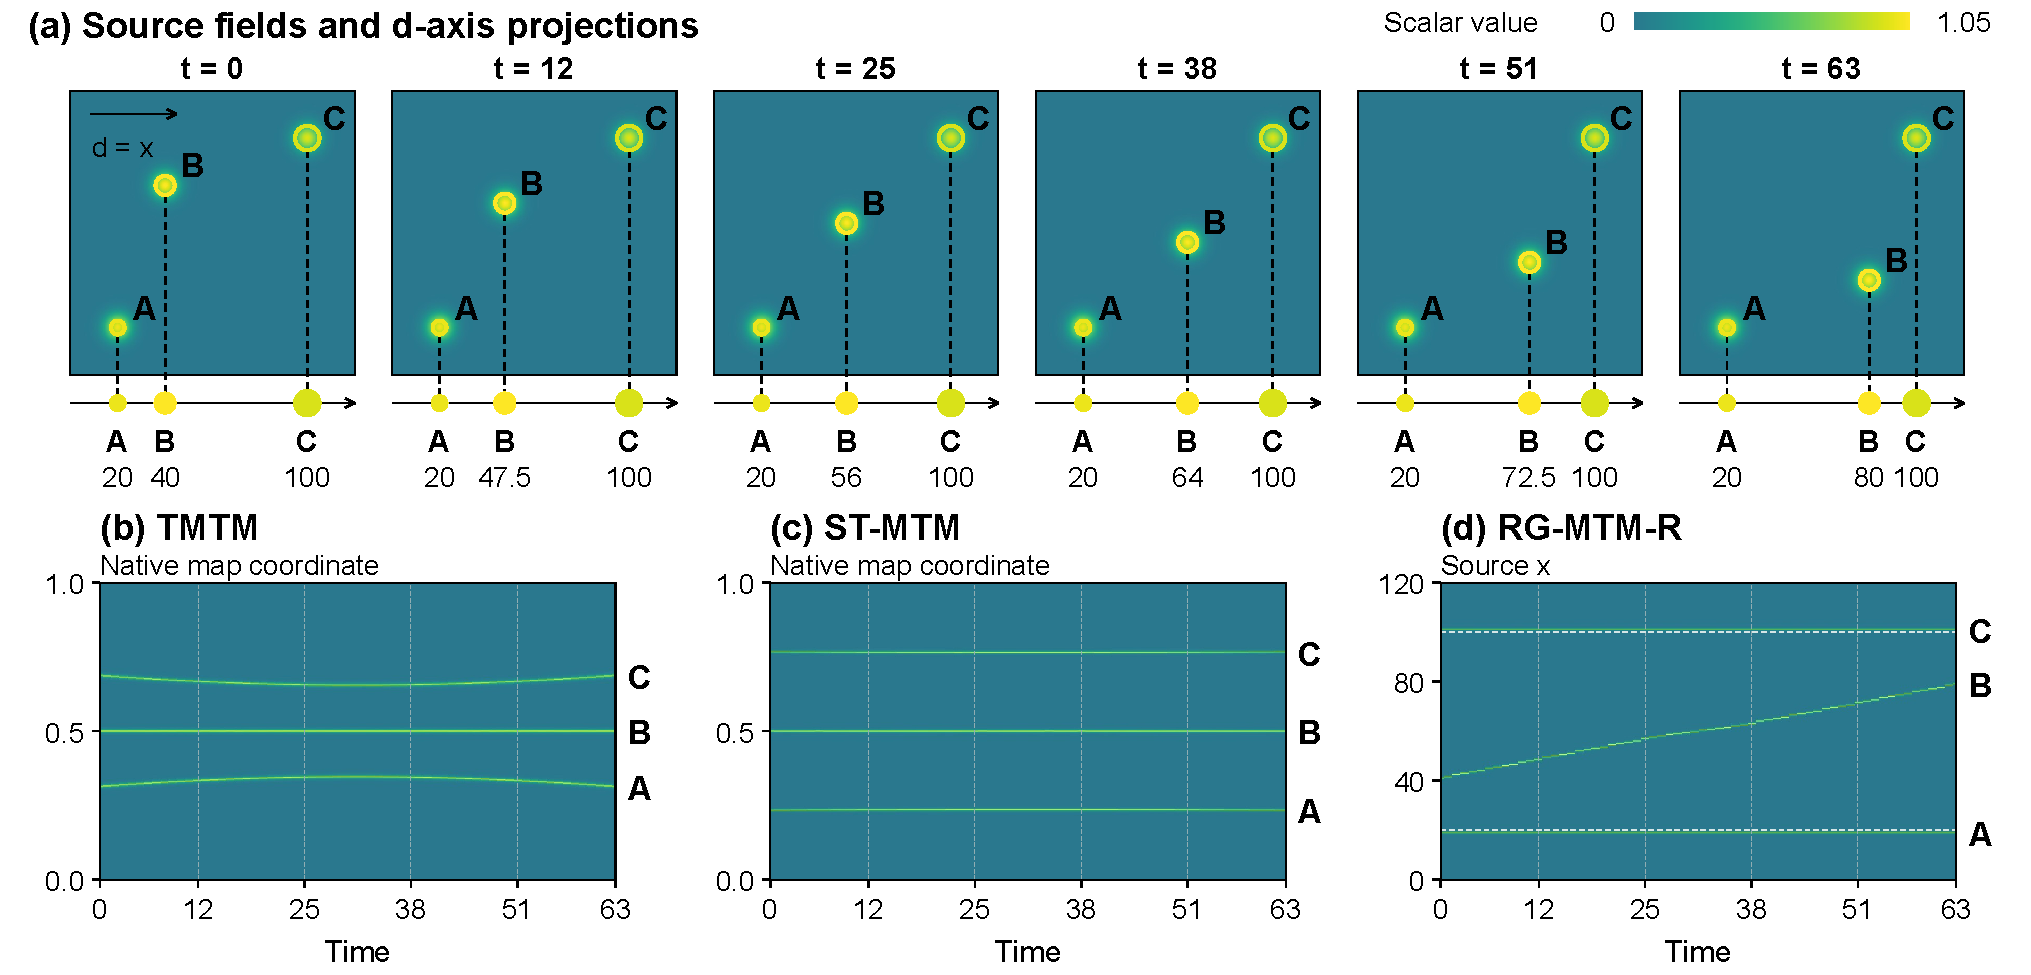
\includegraphics[width=\textwidth]{figures/Fig6.pdf}
\caption{Relative distances and absolute reference position. (a) Six source fields and $x$ projections follow moving $B$ between fixed $A,C$; mirror endpoints preserve pairwise distances while changing horizontal position. (b,c) TMTM/ST-MTM use internal map coordinates. (d) RG-MTM-R uses source $x$ units, with dashed fixed references. Source peaks and temporal bands share a linear 0--1.05 scalar scale. Vertical guides mark source-frame times. All three preserve merge levels; position errors and calibration are reported in Section~\ref{sec:reference_control}.}
\label{fig:bisector}
\end{figure*}
